\documentclass[12pt, letterpaper]{article}
\usepackage[utf8]{inputenc}
\usepackage{caption}
\usepackage{subcaption}
\usepackage{graphicx}
\usepackage{listings}
\usepackage{xcolor}
\def\code#1{\texttt{#1}}
\graphicspath{{./Pictures/}}


\setlength{\parskip}{1em}

%Set up listing env

\usepackage{xparse}



\NewDocumentCommand{\codeword}{v}{\texttt{\textcolor{blue}{#1}}}

\lstset{language=C,keywordstyle={\bfseries \color{blue}}}

\lstset{language=C,keywordstyle={\bfseries \color{blue}}}



\begin{document}

\begin{titlepage}
	\begin{center}
        \vspace*{1cm}	
		\title{Vacuum Meshing Guide}
		\author{William Ellis}
		\date{February 2022}   
		\maketitle
	\end{center}
\end{titlepage}

\maketitle

\section{How Does it Work?}
\subsection{Mesh Skinning}
The skinning algorithm is fairly straight forward. A loop is done over all the elements in the mesh, in which each face/edge of the element is checked to see if it has a neighbour. If the face/edge has no neighbor, then the local face ID is added to a list. This check is done for all the faces/edges. Once completed, the nodes belonging to all the faces/edges in the list are added to their own list, and the connectivity data of these faces/edges is stored in another list. The new skinned mesh is then constructed using the list of nodes and the stored connectivity data.
\begin{figure}[ht]
    \begin{subfigure}{0.48\textwidth}
    	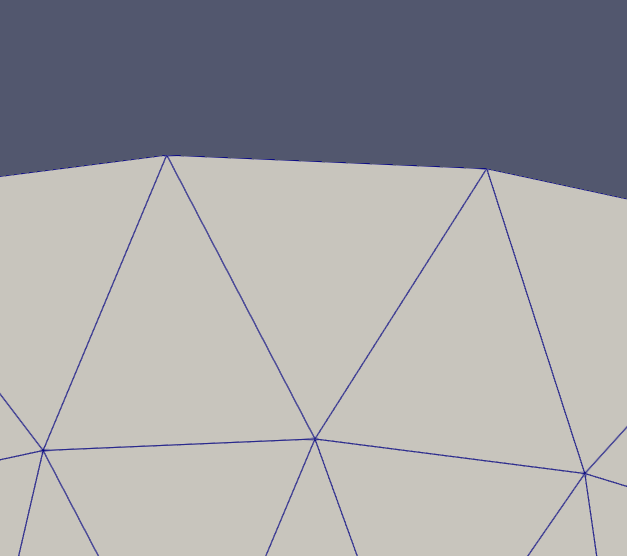
\includegraphics[width=\linewidth]{circleNeighbExample.png}
    \end{subfigure}
    \hspace*{\fill}
    \begin{subfigure}{0.48\textwidth}
    	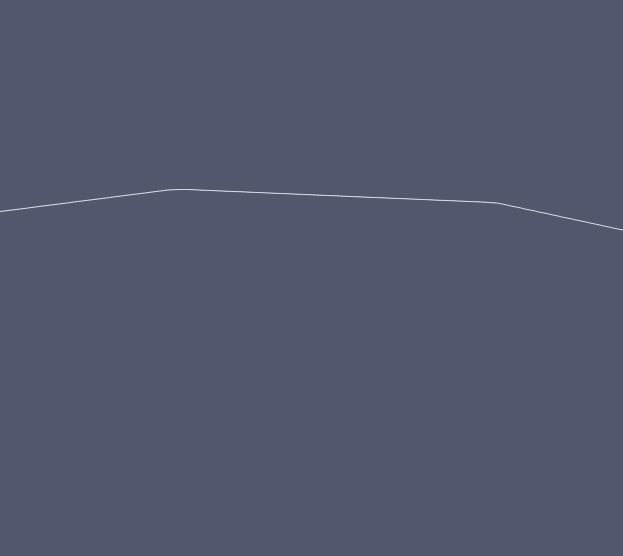
\includegraphics[width=\linewidth]{circleSkinNeighbExample.png}
    \end{subfigure}
    
	\caption{Top down view of a tri mesh. See how the only remaining elements after skinning \
	are the edge elements who had no neighbors.}
	\label{2DSkinExample}
\end{figure}

\subsection{Vacuum Generation}
\begin{figure}
	\begin{subfigure}{0.4\textwidth}
	    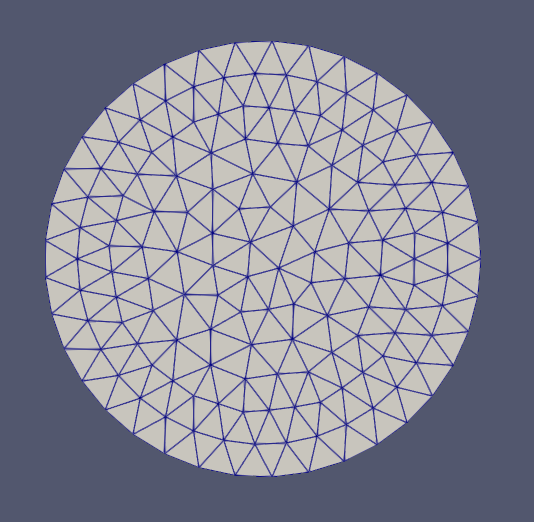
\includegraphics[width=\linewidth]{	processExample/circle.png}
	    \caption{Starting mesh.}
	\end{subfigure}
	\hspace*{\fill}	
	\begin{subfigure}{0.4\textwidth}
	    
\includegraphics[width=\linewidth]{	processExample/skin.png}
	    \caption{Skinned Mesh.}
	\end{subfigure}
	\vspace*{\fill}	
	\begin{subfigure}{0.4\textwidth}
	    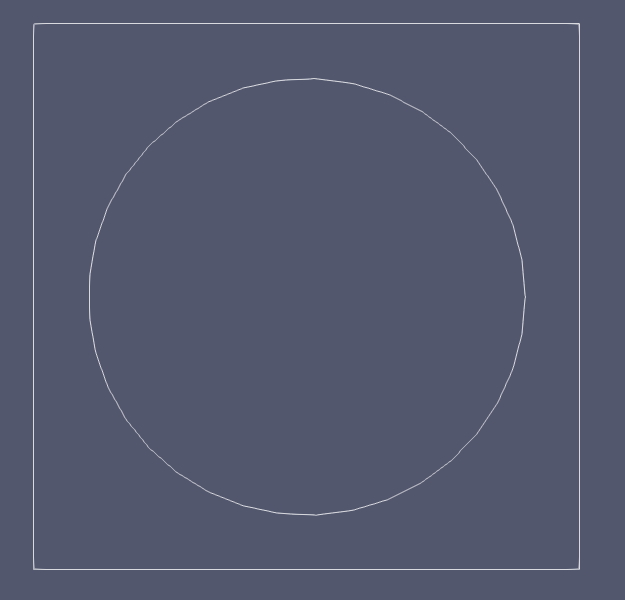
\includegraphics[width=\linewidth]{	processExample/bound.png}
	    \caption{Skinned mesh with boundary generated around it.}
	\end{subfigure}
	\hspace*{\fill}	
	\begin{subfigure}{0.4\textwidth}
	    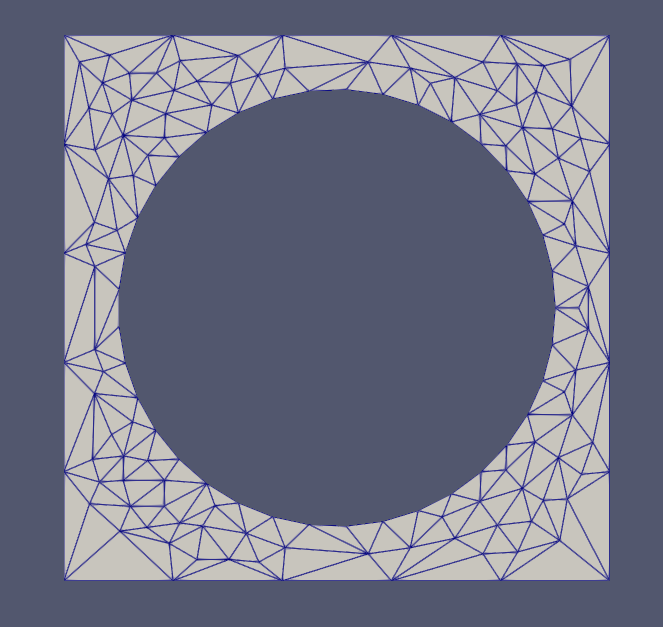
\includegraphics[width=\linewidth]{	processExample/vac.png}
	    \caption{Vacuum mesh generated in the space between the part and the boundary.}
	\end{subfigure}
	\caption{Example process of vacuum generation. This workflow should help\
	show why why the boundary mesh is necessary to generate the vacuum.}
	\label{Boundary Example}
\end{figure}
Vacuum generation is essentially a two step process; boundary generation, and tetrahedralisation. Boundary generation refers to the process of generating a boundary around the skinned mesh. Tetrahedralisation refers to the process of generating tetrahedra (or sometimes tri elements) in a well defined region. Boundary generation is necessary to define the space in which tetrahedralisation will occur. Figure \ref{Boundary Example} helps demonstrate this.

\subsubsection{Boundary Generation}
To define a vacuum region in which tetrahedra can be generated, a boundary surrounding the skinned mesh of the original part must be created. Currently this tool only supports creating cubic boundaries around objects, however if necessary this can be expanded in future. A cubic boundary should suffice for most problems. While Figure \ref{Boundary Example} is useful to visualise need for a boundary mesh, in most cases the user will not be working with 2D planar geometry like the circle shown. It will be more common for a 3D part to be used, which will therefore require a 3D boundary mesh. However, like the skin of a 3D part, this boundary mesh needs to be composed of 2D (tri) elements. Generating a cube composed of 2D mesh elements is easy in dedicated meshing software, but less trivial when you want to do it in your own code. Fortunately a library aptly named "Triangle" exists that enables users to perform Delauny triangulation in the comfort of their own code.Even more fortunately (forunate-lier?), libIGL includes a wrapper around Triangle, making it a simple to add in. It is infact the tool used to generate the tri elements in the 2D example shown in Figure \ref{Boundary Example}. Triangle generates tri elements within planar 2D bounds. Unfortunately, the 2D plane used cannot be defined in 3D as Triangle only takes 2D coordinates (X and Y) in it's arguments. To generate a cube the same face is first generated 6 times. tO allow this face to exist in 3D it is chosen to exist on the XY plane (z=0), so the nodal coordinates do not need to be changed, a column of zeroes is simply added to represent the z coordinate. 

Now that this face exists in 3D, it can be rotated and translated in 3D space. Rotation of a face is can be done by multiplying a selected rotation matrix by the nodal coordinates of all the nodes on that face. The connectivity data for the 2D elements will stay exactly the same, only the location of the nodes must be altered. Translation is once again a simple cased of adding/subtracting an offset to one of the 3 coordinates. Once the faces have been rotated/translated, they can be combined into one mesh, representing the boundary mesh. More information on how the meshes are combined can be found in Section ***. For now it should be made clear that this combination is particularly clean. As all of the faces are copies of one original face, and the edge elements they are generated from can be specified by the user, there are guaranteed to be no hanging nodes.

The generation of a boundary around a coil is a case which has recieved some special attention in this tool. In some FE problems it is necessary for some of the faces of the coil to be coplanar with the vacuum boundary. In this case it is not sufficient to just produce a cubic boundary, as combining the cubic boundary with the coil geometry will results in overlapping nodes and elements at the parts of the coil which need to be co-planar with the boundary. To solve this problem, one of the faces of the cubic boundary has to be produced with cutouts where the coplanar parts of the coil are. The elements and nodes on this boundary must also conform to those already existing on the coil. The other 5 faces of the cubic boundary are created as described prior, and then combined with the remaining one.

\subsubsection{Tetrahedralisation}
Tetrahedralisation refers to the process of generating tetrahedral mesh elements in the space described by the skinned mesh and the boundary mesh. The tool used to generate tetrahedra in this code is Tetgen. This is the tetrahedral analogue to the aforementioned Triangle library. tetgen 

Tetgen includes many built it options that can be used to manipulate its behavoir. 

\subsection{Full Mesh Generation}
\subsubsection{Combining Meshes}
\subsubsection{Boundaries}
\section{Building}

\section{Using}
\subsection{Using the examples}
There are three examples built in to the repo. These examples utilise  the functionality found in the library to different extents, and should be enough for most users to do what they need.

\subsubsection{skinner}
The first example, the source of which can be found in problems/skinner.cpp, is an example of how to get the skin of a mesh. This example loads in an input mesh given by the user and utilises the function \codeword{getSurfaceMesh} to obtain the skin of the input mesh. This can be used with meshes composed of 2D or 3D elements. In the 2D case, the skinned mesh will be composed of 1D edge facets, representing the boundary of the 2D boundary. In the 3D case, the skinned mesh will be composed of 2D facets. 

\begin{figure}
	\begin{subfigure}{0.48\textwidth}
		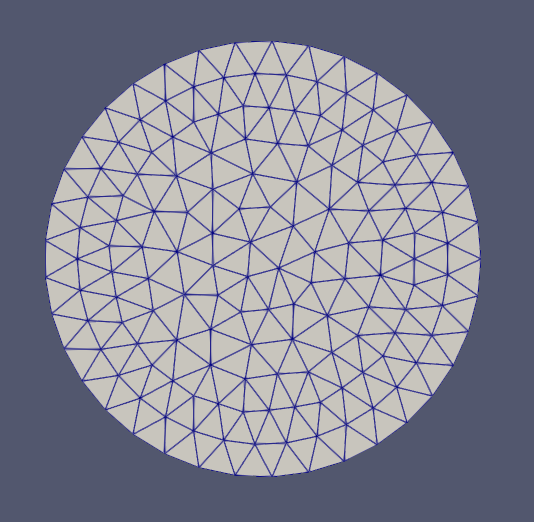
\includegraphics[width=\linewidth]{processExample/circle.png}
		\caption{Before}
	\end{subfigure}
	\hspace*{\fill}	
	\begin{subfigure}{0.48\textwidth}
		
\includegraphics[width=\linewidth]{processExample/skin.png}
		\caption{After}
	\end{subfigure}	
	\caption{Example of skinning a mesh composed of 2D facets.}
	\label{2DSkinningComp}
\end{figure}

For example, if you had a mesh called `myMesh.e`, from the command line you could enter 
\begin{lstlisting}[language=bash]
	./build/examples/skinner -i Meshes/myMesh.e
\end{lstlisting}
to skin a mesh called myMesh. This should successfully save a mesh called MyMesh\verb|_|skin.e in the directory where the command was called from. 

\subsubsection{Generate Vacuum}
The second example included in the repo 

\subsection{Using the library}
As previously mentioned, the functionality found in this repo is built into a library called "VacuumMeshing". The example executables are linked to this library in order to utilise the funtionality. There is no reason that this library couldn't be linked to any of your own projects. Within the repo, naviating to "./VacuumMeshing/CMakeLists.txt" will show you how the library is built. The libIGL libraries that are linked in when the library is created have PUBLIC "inheretence". This means that any targets depending on this library will automatically be linked in with the necessary libIGL libs. This saves the user (you) having to mess around with ligIGL includes/libs. The MPI lib linked in with the library is set as PRIVATE, so that when building your own projects they will NOT link against the MPI version used to build the VacuumMeshing library.

\end{document}
